\chapter{The Schneckenhaus System}
\textit{In this chapter, I will address the topics of stress management system (Schneckenhaus) development. Discusses the development of the system and all elements which I have been used to implement the system for stress management at the  workplace  in  particular  for people with stress overflow}
\vspace{5mm}

A stress management system named \textbf{Schneckenhaus} has been developed to achieve the aim and objective of the research which is to decrease the stress level and empower the users through this system. 

Feeling stressed most of the time in the workplace which I have focused on in the initial phase of the thesis is a stress overflow. An extensive literature review has been done in chapter 2: Related work to get ourselves aware of the problem in detail before we started developing the system.

The main goal of developing this system is to create a user's friendly stress management system that can manage stress when they overflowed. In the next section of this chapter, I will explain details about the Schneckenhaus system design.

\section{System Design}
System design is the process of designing the elements of a system such as the architecture, modules and devices, the different interfaces of those components and the data flowing through that system. 

The aim of the system design process in my thesis is to provide sufficient detailed data and information about the system, and this system elements to allow implementation consistent with the architectural entities as described in system architecture models and views.

Making system design more specific firstly I design \acf{UX} and then I develop \acf{UI}.
\subsection*{\acf{UX}}
Designing user experience is a human-first process of product design. A cognitive scientist and co-founder of the Nielsen Norman Group Design Consultancy, Don Norman has been credited with coining the term "user experience" in the late 1990s. He defines it this way:

    \say{User experience encompasses all aspects of the end-users interaction with the company, its services, and its products.}
– Don Norman, Cognitive Scientist \& User Experience Architect \citep{Norman1988TheThings}

I use persona analysis outcome (mentioned in section:\ref{Persona Analysis Outcome}) and paper prototype findings (mentioned in section:\ref{Findings of Paper prototype}) to design \acf{UX}  for our stress management system \textbf{Schneckenhaus}. 

\subsubsection*{User Experience Design Process}
User experience design process is an iterative method that helps me continuously improve and polish my designs. In the process, I go through different stages repeatedly while evaluating my designs on each stage. Each stage involves relevant stakeholders in my thesis that take part in the process to make my thesis highly efficient and usable.

Schneckenhaus system UX design process involves following six stages based on: \citep{Minhas2018UserPlanet}

\begin{itemize}
    \item \textbf{Understand:} Understand requirements create user personas define use case.
    \item \textbf{Research:} Analyze related work research latest UX trends
    \item \textbf{Sketch:} Gather ideas draw sketches and wireframes evaluate and re-draw
    \item \textbf{Design:} Design Images, Create prototypes, Define UX guidelines
    \item \textbf{Implement:} Implement functionally build experience
    \item \textbf{Evaluate:} Perform usability testing, identify improvements.
\end{itemize}

Considering \acf{UX} In the next section we will discuss about \acf{UI} development.

\subsection*{\acf{UI}}
Schneckenhaus system UI is being developed in the android platform using the latest coding language, standards, and practices of Android Programming. The programming language which has been used to develop this app is Kotlin. 

According to Kotlin's official website "Kotlin is a cross-platform, statically typed, general-purpose programming language with type inference. Kotlin is designed to interoperate fully with Java, and the JVM (Java Virtual  Machine) version. 'In Google I / O 2017, Google officially supported Kotlin for mobile development in Android. And the company also encouraged Android Developers to start developing their apps in Kotlin. 

For making the system more user-friendly, I developed a single app solution and integrate all functionality of the Schneckenhaus system. In the next section, I will discuss the system overview.

\section{System Overview}

\begin{figure}[hbt!] 
  \centering
  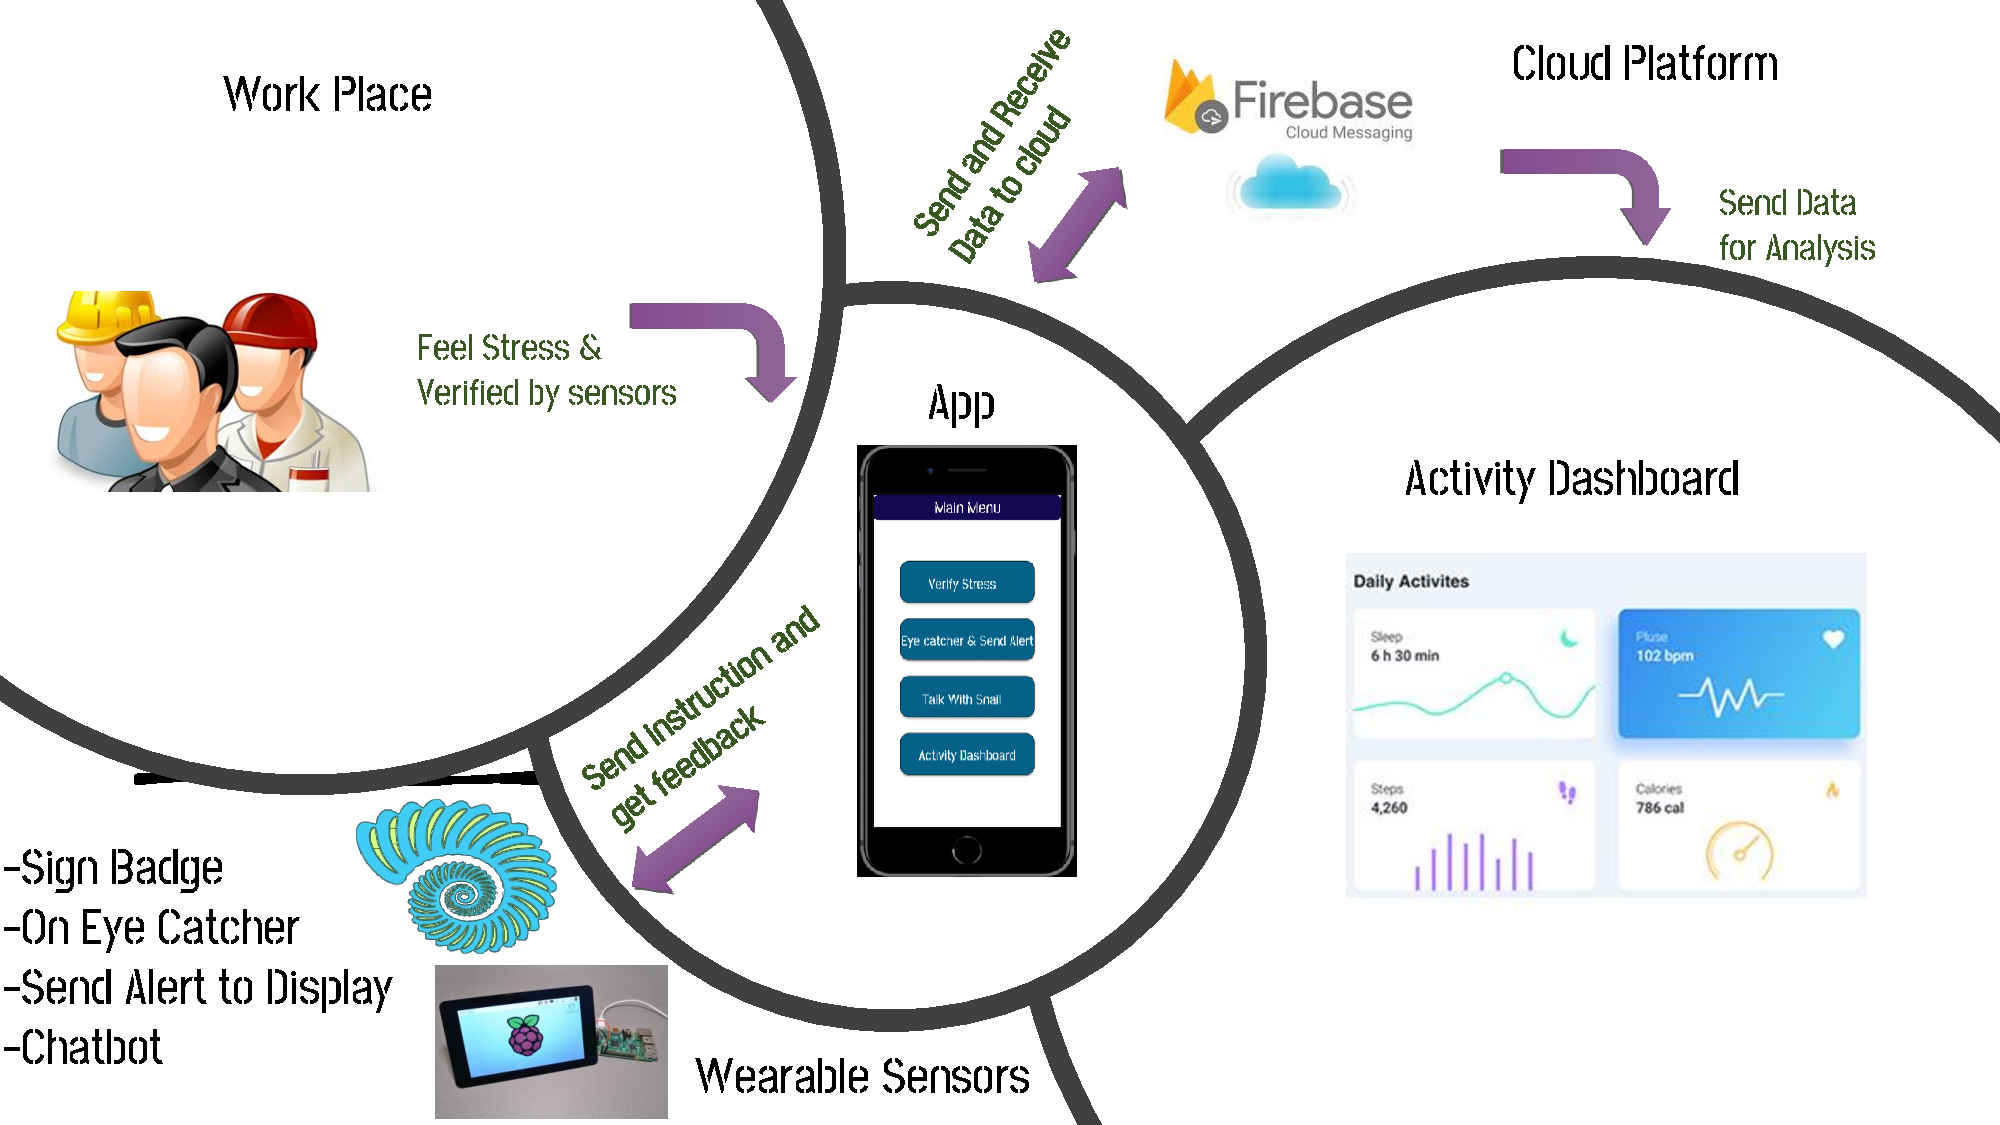
\includegraphics[width=1.0\linewidth]{chap4/image4/Overview.pdf}
  \caption[Schneckenhaus system overview ]{Schneckenhaus system overview\index{Hasnain}}
  \label{fig:overview_Stress}
\end{figure}
Schneckenhaus system combined with android app, multiple wearable sensors, IoT devices, physical eye-catcher, chatbot, activity dashboard. In figure :\ref{fig:overview_Stress} draw an ecosystem, how the system will work and will be the reaction and communication between components of the system. Let me explain the system working process. This system is suitable for the workplace environment and for people who have stress overflow.

In the workplace, the employee has lots of activity throughout the day. They do not always feel stressed. when they feel stressed my Schneckenhaus system area start from that point. I developed an android application as \acf{UI} for my system. This app main menu (See fig: \ref{fig:main_menu}) have the following four activity button which is connected with all components and tools of the system. 

\begin{enumerate}
    \item Verify stress
    \item Eye catcher and send Alert
    \item Talk with snail
    \item Activity Dashboard
\end{enumerate}

\begin{figure}[hbt!] 
  \centering
  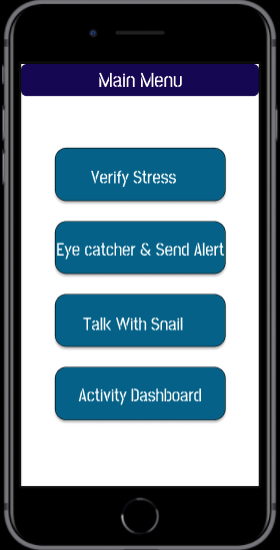
\includegraphics[width=0.4\linewidth]{chap4/image4/SC2.png}
  \caption[Schneckenhaus System UI app Main Menu ]{Schneckenhaus System UI app Main Menu\index{Hasnain}}
  \label{fig:main_menu}
\end{figure}

\subsubsection*{Verify stress}
In a stressed situation, the employee opens the Schneckenhaus app and press Verify stress activity button. The system will connect immediately to the two components of this activity. one is heart rate sensor via smartwatch another one is \acf{SpO2} for check the current heart rate and oxygen level of blood. this two components result Will verify user stress level with feelings. 
\subsubsection*{Eye catcher and send Alert}
when system recognized user is in stress app suggest to go for the next option which is an Eyecatcher and send an alert. This activity has three component. First one is a special sign badge, the user has to wear this badge on their shirt. the second one is Eyecatcher, it's a Schneckenhaus symbolic lightbox with two colour light green and blue. User can control the light via my Schneckenhaus app. Green light means no stress and blue light means stress overflowed which I found from persona analysis in chapter \ref{Persona Analysis Outcome}. then send customize massage or emoji to wireless display to inform concerns.
\subsubsection*{Talk with snail}
After acknowledging to the surrounding environment, the user needs to distress his stress. On this point, my system will suggest user Talk to Snail. Snail is the name of my chatbot. Snail name comes from the English name of  Schneckenhaus. In this system, Snail is the virtual assistant and trusted friend. In the back-end, it's connected with google Dialogflow API. This API use \acs{NLP} and \acs{AI} process conversion model. The snail will instruct user for doing some physical activity (e.g take five deep breath for 30 seconds) which will make use relax. Its also interact with the user-based conversation.
\subsubsection*{Activity Dashboard}
User, all activity throughout the system with the above mention activity will be recorded and send to the cloud server. This activity data use for the source of my system dashboard for visualization. When a user feels relax or does not have overflowed stress, they can check their activity. The user also can learn from his activity and take appropriate action if needed. This activity dashboard developed in React.js framework. React.js is one of the popular JavaScript frameworks to develop web-based visualization.

In the next section of this chapter, I will explain the Schneckenhaus system UI activity and components in details.

\section{Verify Stress}
\begin{figure}[hbt!] 
  \centering
  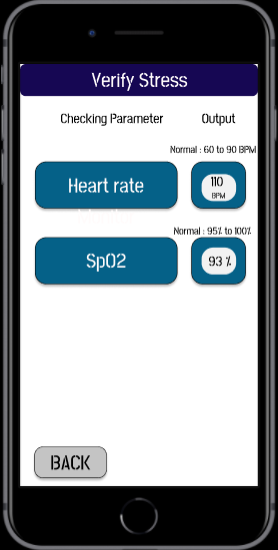
\includegraphics[width=0.4\linewidth]{chap4/image4/sensor.png}
  \caption[Verify Stress activity Component ]{Verify Stress activity Component \index{Hasnain}}
  \label{fig:Verify_Stress}
\end{figure}
In this activity, I designed and developed a system  to verify the psychophysiological signals monitoring stress during workplace and send data to cloud for analysis. 

In the workplace when you feel the stress they can immediately go to the app then press verify stress option. Figure: \ref{fig:Verify_Stress} shows the UI of Verify Stress Activity.The app will give two different types of health data from \acs{IoT} sensors.

\begin{itemize}
    \item 1. Heart rate sensor
    \item 2. \acf{SpO2} Sensor
\end{itemize}

In measuring health status, sensors and smartphones usually imply: collecting sensor data; providing user support through a display with the measured values; sharing information; ensuring low power devices, wear-ability, accuracy, durability and system reliability.

\subsection{Smart watch Heart rate sensor}
\begin{figure}[hbt!] 
  \centering
  \subbottom[Front view]{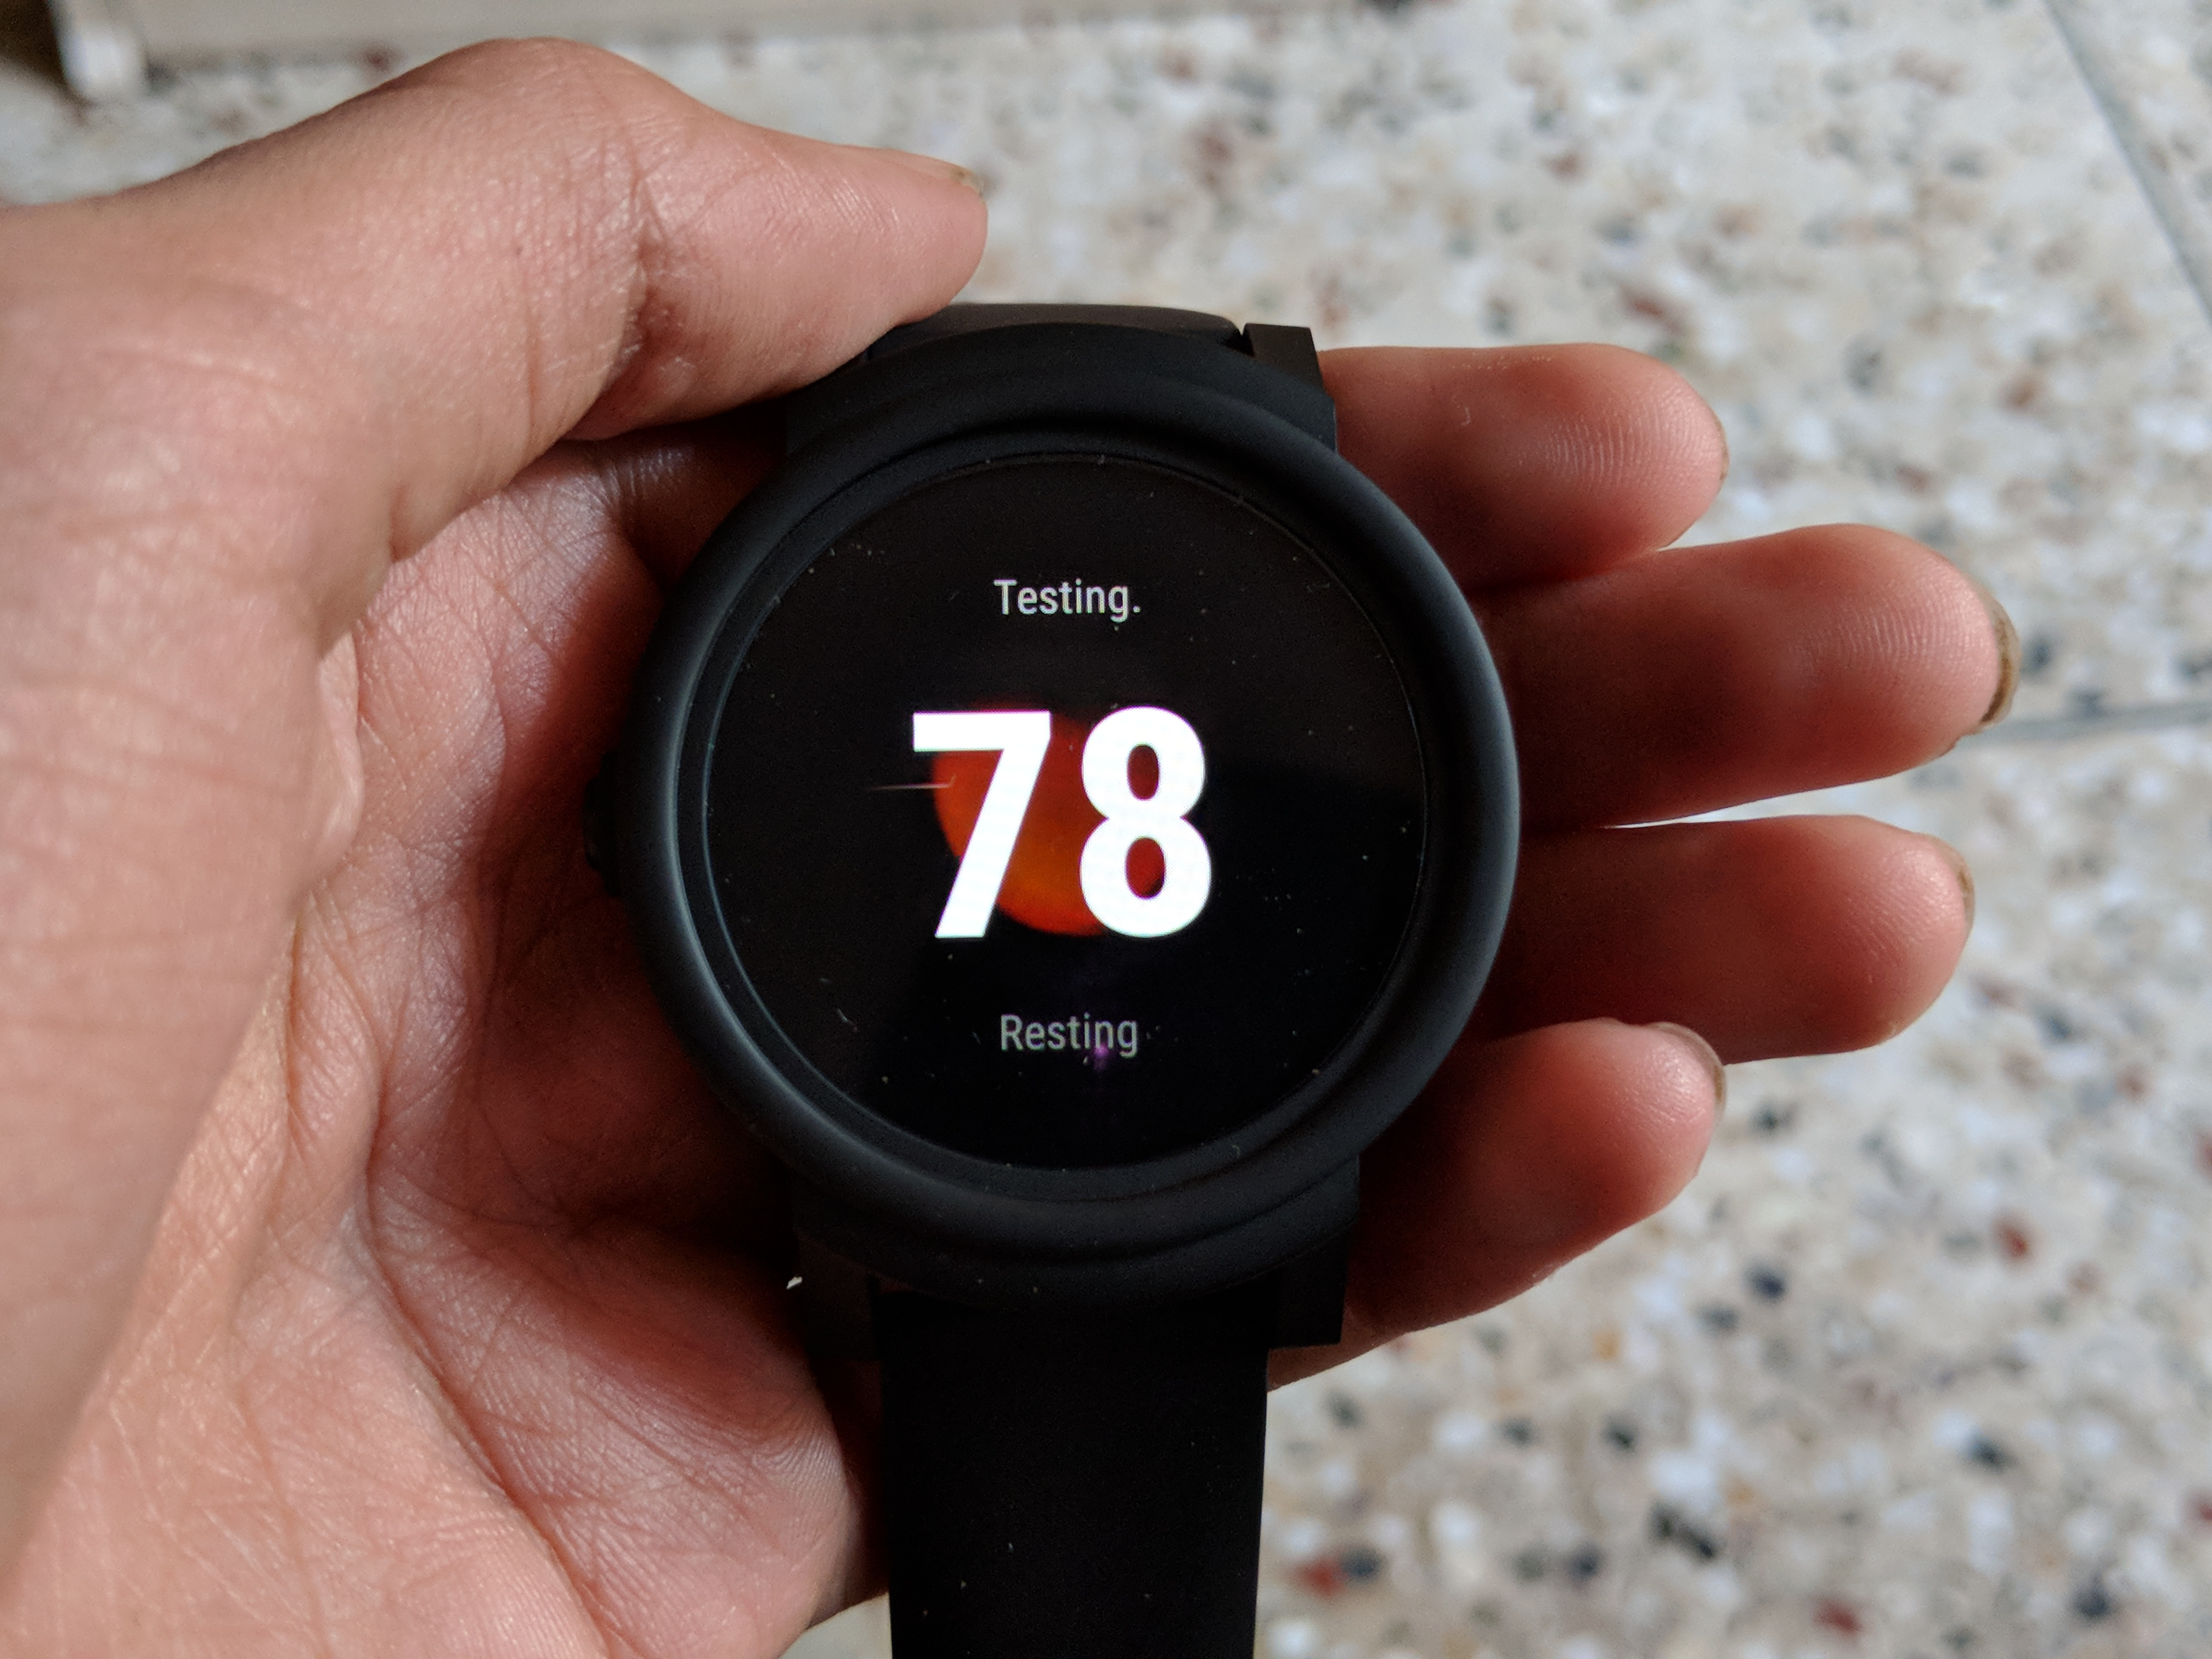
\includegraphics[width=0.45\textwidth]{chap4/image4/tikwatch.jpg}}\qquad
    \subbottom[Back side sensor view]{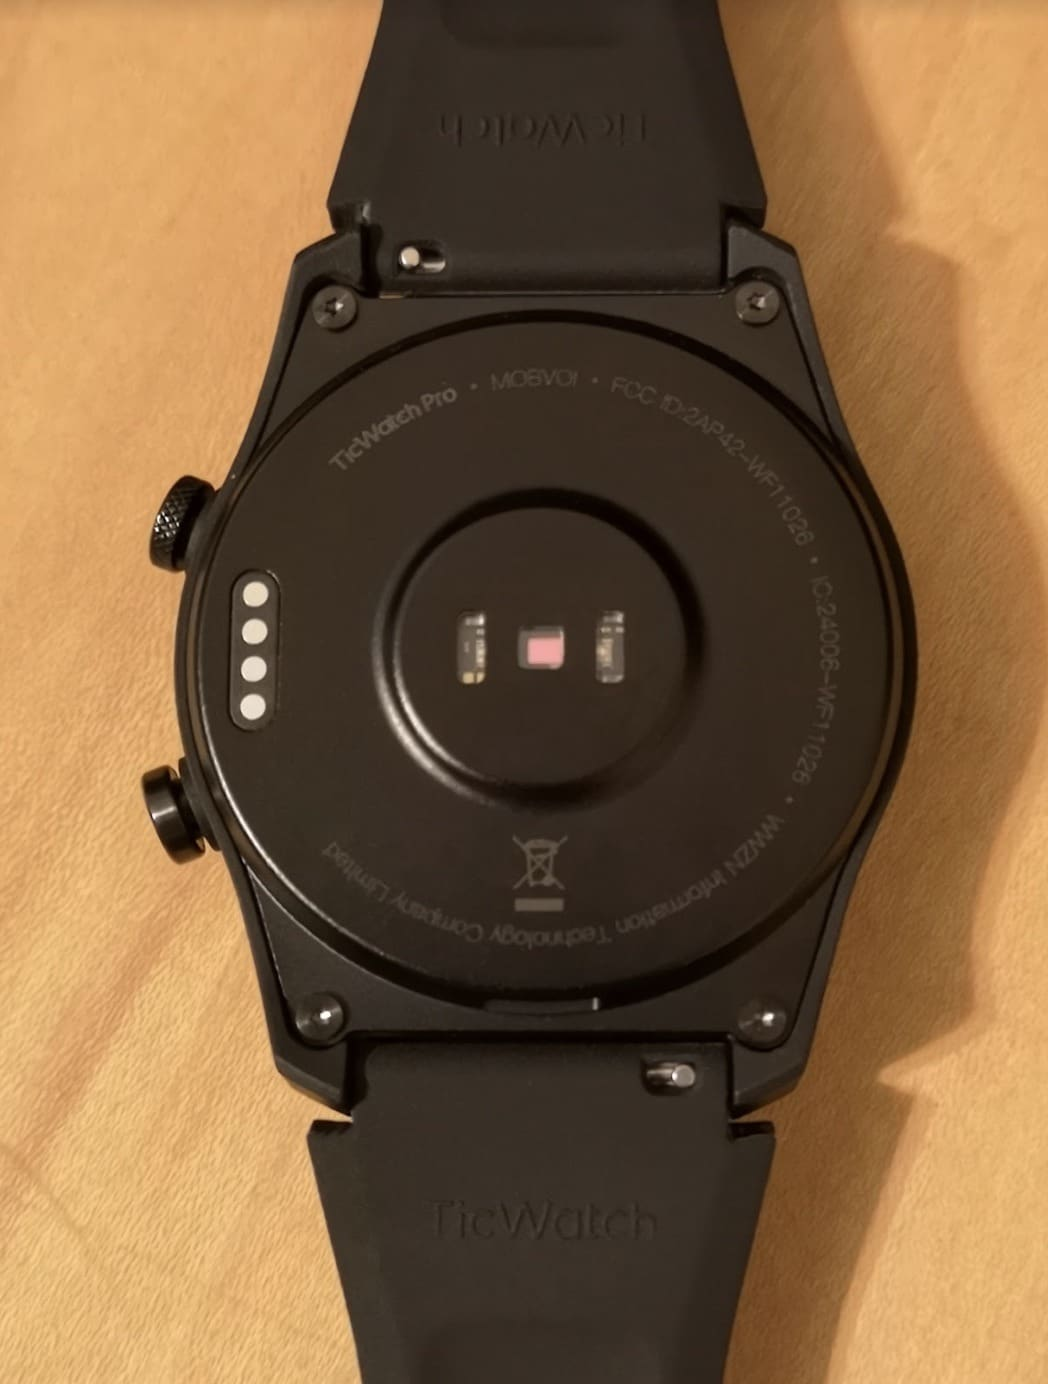
\includegraphics[width=0.26\textwidth]{chap4/image4/tikwatch1.jpg}}
  \caption[Ticwatch Smartwatch S2, Wear OS ]{Ticwatch Smartwatch S2, Wear OS\index{Hasnain}}
  \label{fig:Ticwatch}
\end{figure}
One of the main challenges is the design of a wearable, low-power, reliable and precise \acs{IoT} system. Commercial solutions also satisfy the criteria set out above.  One such solution is the fully wearable Ticwatch Smartwatch S2, Wear OS (shown in Fig.\ref{fig:Ticwatch}). The device has a Bluetooth module which allows communication with a suitable mobile application. This comes with no Google Fit API, as most commercial solutions do, and is thus programmable and customise able. Therefore, for real-time monitoring, further analytic, biofeedback, or integration with other educational services, there is possible to collect sensor data and store it in the Firebase database.

To maintain homeostasis, physical or mental imbalance induced by harmful stimuli can induce stress. The sympathetic nervous system is hyperactivated during chronic stress which causes physical, psychological, and behavioural abnormalities. There is currently no accepted standard for assessing stress. This analysis aimed to survey studies that provide a basis for choosing variation in the \acf{HR} as a measure of psychological stress.\citep{Kim2018StressLiterature}

User heart rate is changing from one minute to another. It depends on whether you stand or lie, move around or sit still, stressed or relaxed. Nonetheless, the restful heart rate continues to be steady every day. The usual heart rate resting range is between 60 and 90 beats per minute, anywhere. Over 90 is generally considered high.\citep{LeWine2011IncreasePublishing}
\subsection{\acf{SpO2}}
\acs{SpO2} stands for saturation of the peripheral capillary oxygen. It estimates how saturated the oxygen in your blood is. A safe, fit person usually sees a \acs{SpO2} ranging from 95\% to 100\%. Illness, altitude, heart disease, inhalation of smoke all have \acs{SpO2} effect.\citep{Sly2019ManagingBiostrap}
\begin{figure}[hbt!] 
  \centering
  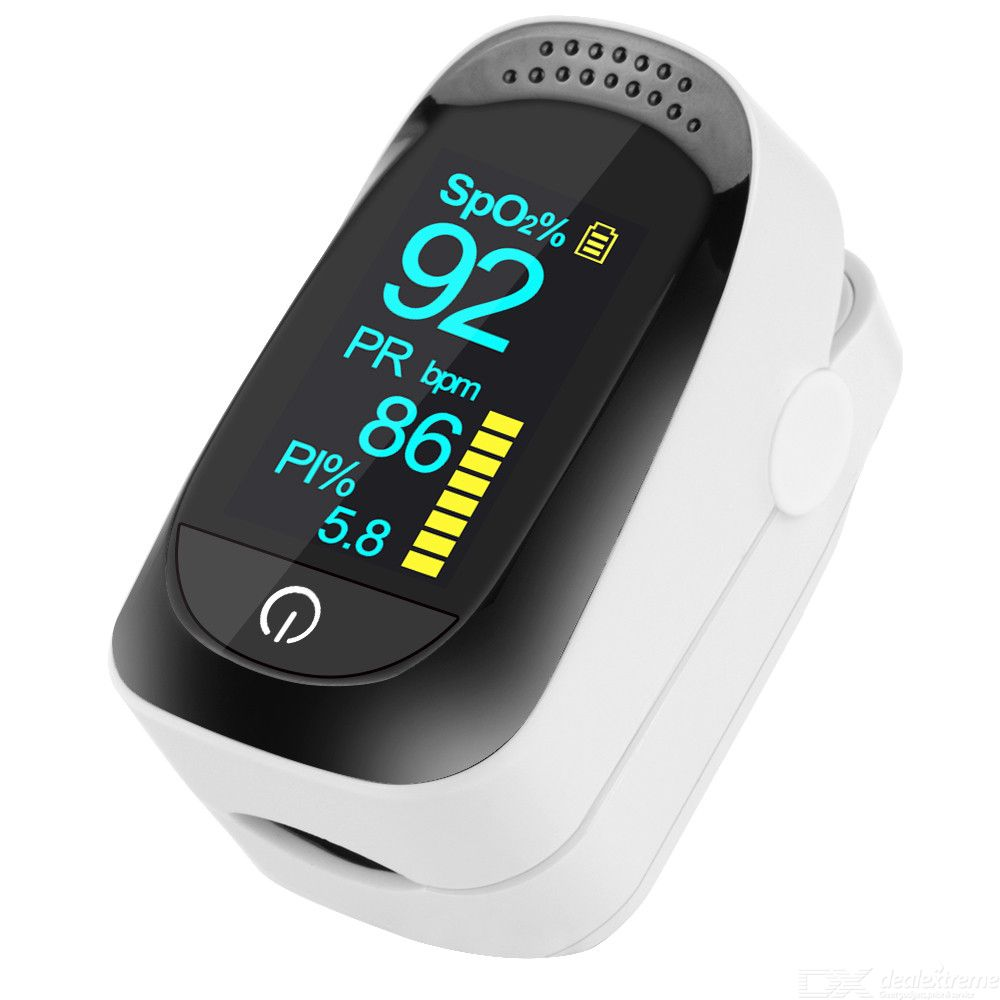
\includegraphics[width=0.5\linewidth]{chap4/image4/spo22.jpg}
  \caption[\acf{SpO2}]{\acf{SpO2}(source:\cite{Teleportz2019A2Shop}\index{Hasnain}}
  \label{fig:spo2}
\end{figure}
 Measure of \acs{SpO2} may not vary as much as user resting heart rate and HRV, but a sudden drop is often an indication of stress. Traditionally, athletes who train at higher altitudes track \acs{SpO2} to help make sure they get enough oxygen. This is an easy metric to track with the correct device along with the resting pulse.

\acs{SpO2} instant measurement device shown in figure:\ref{fig:spo2}. In this activity, I use this device for verifying the stress with personal feelings. And send data to the cloud for further analysis and visualization.

\section{Eye catcher and send Alert}
This activity is the part of Symbolic Representation for Others. Symbolic representation is a communicative activity that distinguishes human beings from other species and brings them together within cultures and other social groups. This section explores symbolic representation in our study, and restrict our development to symbolic representation in the context of external symbols used in contact with others.
\begin{figure}[hbt!] 
  \centering
  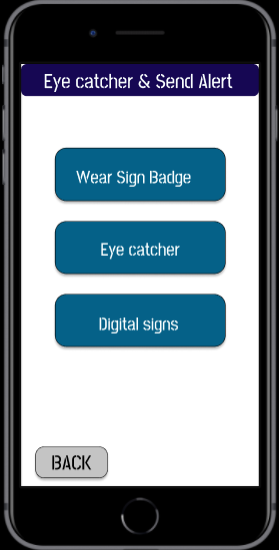
\includegraphics[width=0.4\linewidth]{chap4/image4/eye.png}
  \caption[Symbolic Representation for Others activity Component ]{Symbolic Representation for Others activity Component\index{Hasnain}}
  \label{fig:Sign}
\end{figure}
I used Three types of Symbolic representation for alert surrounding at work place.
\begin{itemize}
    \item Special Sign Badge
    \item Eyecatcher
    \item Digital signs to Wireless display
\end{itemize}

\subsection{Special Sign Badge}
In this activity, I use \textbf{Schneckenhaus} symbol badge as a metaphor of stressed condition. A stress status symbol is a visible perceived, external denotation of one's social position and perceived social status indicator.\citep{Cherrington1994OrganizationalBehavior} Many luxury goods are often considered status symbols. A status symbol is also a sociological term relating to how individuals and groups interact and interpret various cultural or stressed symbols, as part of social and sociological symbolic interactionism.
\begin{figure}[hbt!] 
  \centering
  
\includegraphics[width=0.4\linewidth]{chap4/image4/logo1.png}
  \caption[Schneckenhaus symbol sign badge ]{Schneckenhaus symbol sign badge\index{Hasnain}}
  \label{fig:Sign_badge}
\end{figure}
In this activity, I use special sign badge(see figure \ref{fig:Sign_badge} for acknowledging other collages about user current status. It should be previously circulated among the workplace from \acs{HR}.
\subsection{Eye catcher}
Based on dictionary Eye catcher means a thing that attracts attention. In our thesis, we use eye-catcher as a box (see figure \ref{fig:eye}). We made this box in our FAB lab and design with our Schneckenhaus symbol. Inside the box, we used two-colour LED, Green and Blue. This Led control by stress management app.  When the user has stressed condition too high, they should turn on the blue LED. When stress condition is a normal condition the switch back to green. 
\begin{figure}[hbt!] 
  \centering
  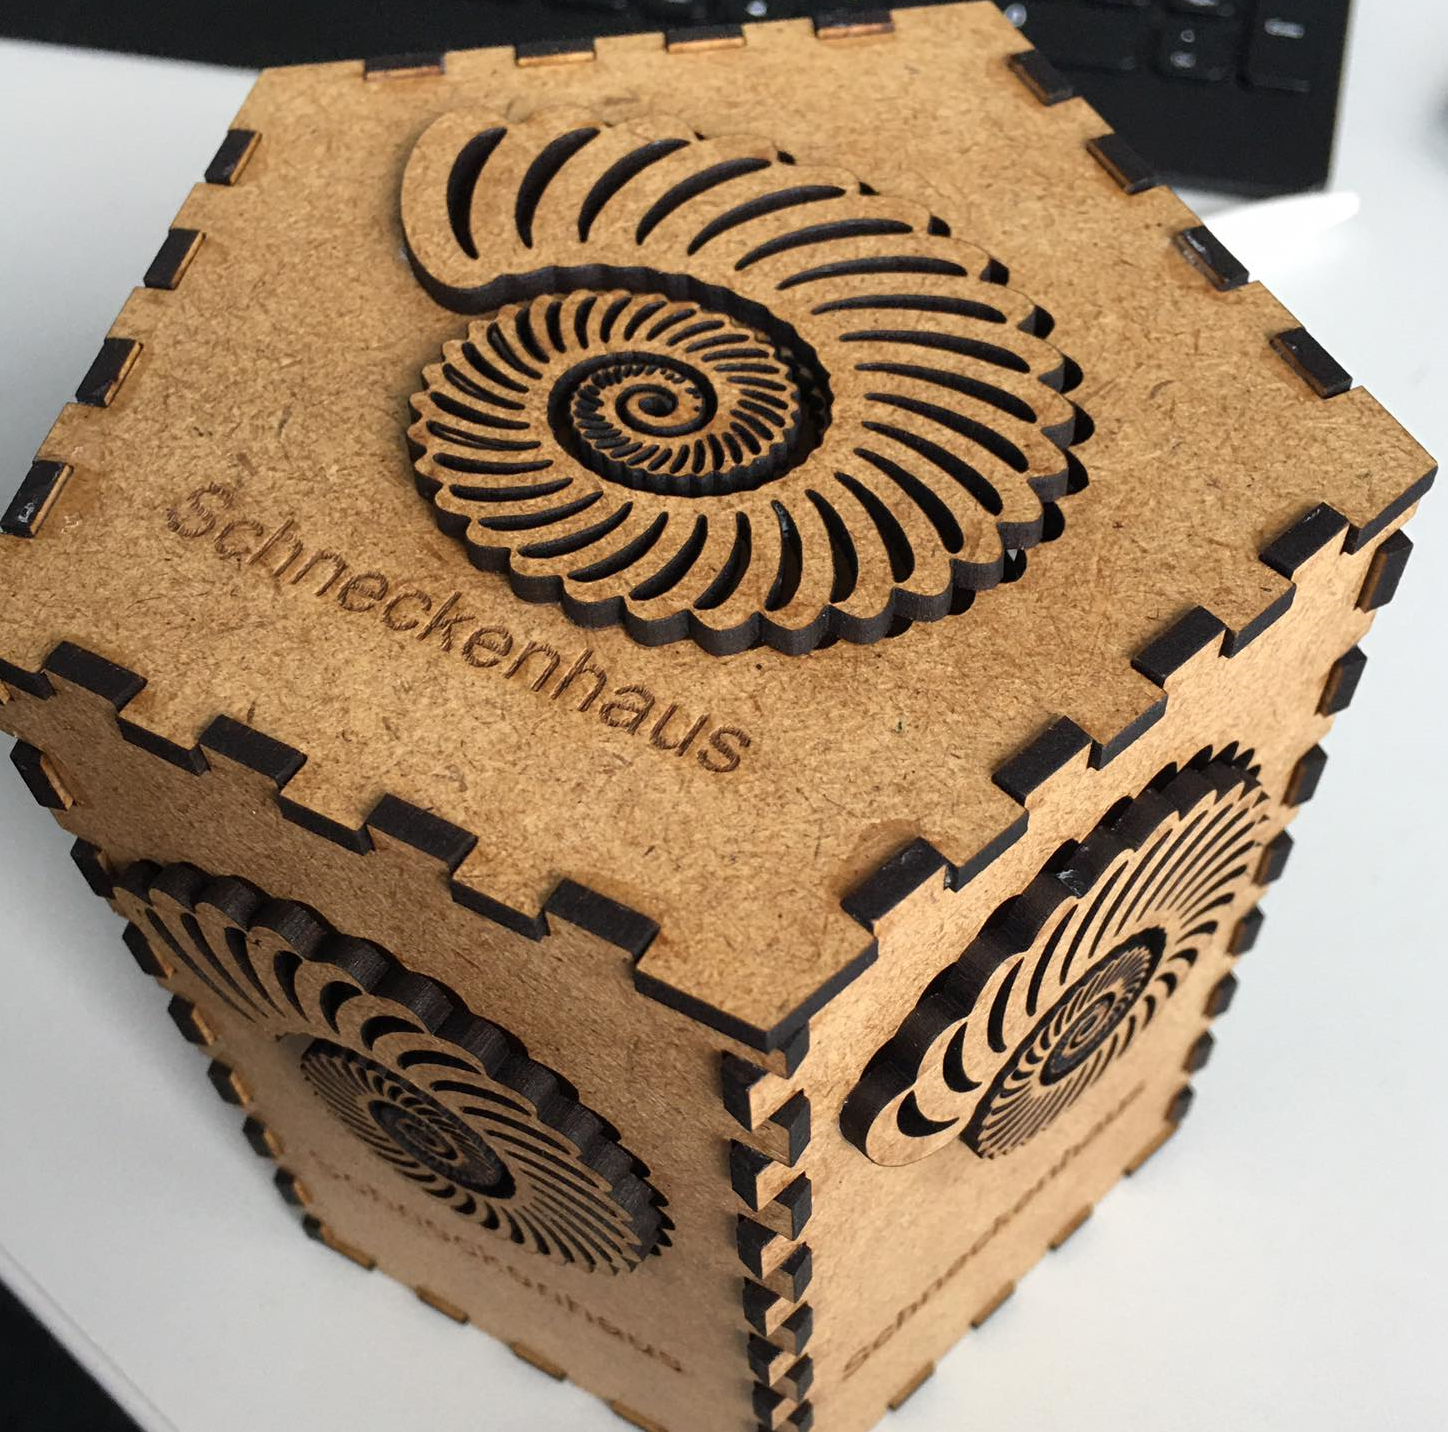
\includegraphics[width=0.5\linewidth]{chap4/image4/skn2.png}
  \caption[Eye catcher ]{Eye catcher\index{Hasnain}}
  \label{fig:eye}
\end{figure}
For communication with Schneckenhaus app with LED switching control we used NodeMCU device.

NodeMCU is an open-source \acs{IoT} platform which is low cost. Initially, it included firmware running on Espressif Systems ' ESP8266 Wi-Fi SoC, and hardware based on the ESP-12 module. Later, support was added for the 32-bit ESP32 MCU(see figure \ref{fig:node}.
\begin{figure}[hbt!] 
  \centering
  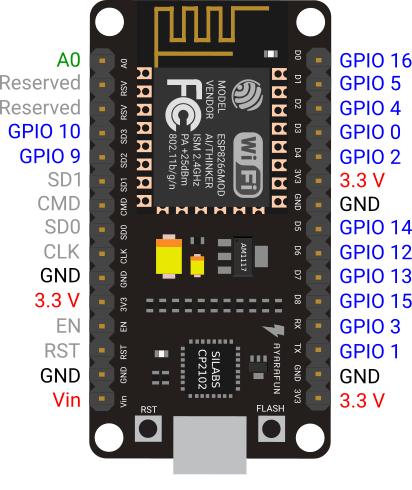
\includegraphics[width=0.5\linewidth]{chap4/image4/Node.png}
  \caption[NodeMCU with ESP8266 pinout ]{NodeMCU with ESP8266 pinout\index{Hasnain}}
  \label{fig:node}
\end{figure}
For writing code inside the NodeMCU used Arduino IDE. See below code. It explain how I wrote code to control LED through our Schneckenhaus app. I attached full code details in appendix. 

\begin{lstlisting}
// Read the first line of the request
  String req = client.readStringUntil('\r');
  Serial.println(req);
  client.flush();
  
  // Match the request
  int val;
  if (req.indexOf("/gpio/0") != -1)
    val = 0;
  else if (req.indexOf("/gpio/1") != -1)
    val = 1;
  else {
    Serial.println("invalid request");
    client.stop();
    return;
  }

  // Set GPI0 according to the request
  digitalWrite(D4, val);
  
  client.flush();

  // Prepare the response
  String s = "HTTP/1.1 200 OK\r\nContent-Type: text/html\r\n\r\n<!DOCTYPE HTML>\r\n<html>\r\nGPIO is now ";
  s += (val)?"high":"low";
  s += "</html>\n";

  // Send the response to the client
  client.print(s);
  delay(1);
  Serial.println("Client disonnected");

  // The client will actually be disconnected 
  // when the function returns and 'client' object is detroyed
}
\end{lstlisting}

\subsection{Digital signs to Wireless display}
\begin{figure}[hbt!] 
  \centering
  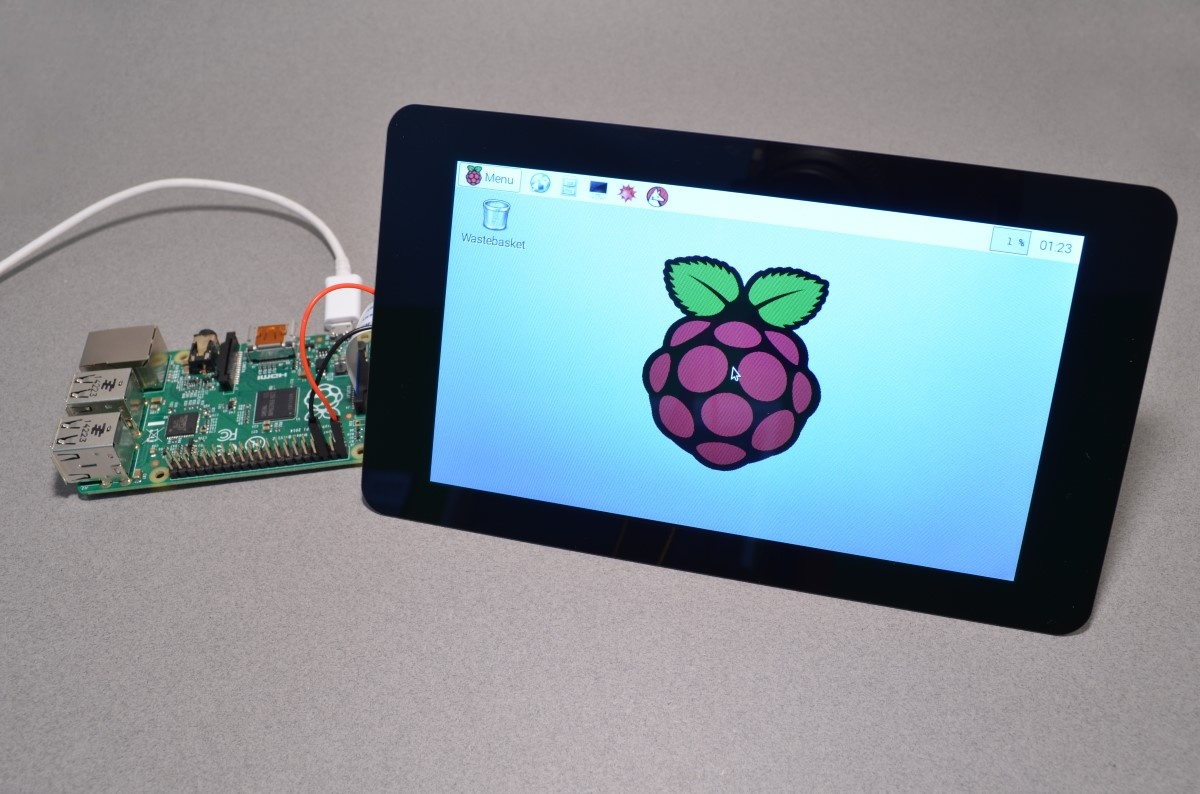
\includegraphics[width=0.5\linewidth]{chap4/image4/dipl.jpg}
  \caption[Raspberry PI Wireless display ]{Raspberry PI Wireless display\index{Hasnain}}
  \label{fig:PI_disp}
\end{figure}
For this activity, I use digital signage concept to make wireless display for send alert or massage to respective person in the work place.

The emergence and ongoing development of \acf{DS} systems give rise to an increasing number of such systems ' technological capabilities. While these technological capabilities have attracted considerable attention in computer science research, scarce studies are exploring their application and effect.  Marketing, and retailing in particular, represents an applied science which could benefit from \acf{DS}.  Some studies demonstrate in support of this assumption that the presence of \acs{DS} showing emotional content creates favourable shopping experiences and positively influences consumer behaviour.\citep{Bauer2018ResearchRetail}

Digital signs help people with Stress Overflowed to communicate better with their colleague and managers. Teams can use digital signs on their office walls to show special massages. Digital signage is an innovative medium of communication due to its always-on existence, allowing individuals to easily view and communicate with digital signs during the hustle and bustle of their busy days.

I need digital signage software to launch the digital signage on Raspberry PI. This software helps me to change my display screen and to manage the content. It is, however, a critical component of any successful strategy for digital signage. \acs{DIY} digital signs can be complicated and time-consuming to keep up-to-date without digital signage management software.

I use Screenly OSE in this activity for contents management. I will explain how to deploy the Screenly OSE software for open-source digital signage using balenaCloud. With balenaCloud, users can use the Public URL feature to manage their Screenly OSE powered digital signs from anywhere with an internet connection. This remote management is a game-changer for stress management in the workplace, as it is.

\section{Interactive Chatbot}
A chatbot is a \acf{AI} program that simulates interactive human conversation using key pre-calculated user phrases and auditory or text-based signals. Chatbots are often used for basic customer service and marketing systems which frequent hubs of social networking and \acf{IM} customers. They too are often included in operating systems as intelligent virtual assistants.
\begin{figure}[hbt!] 
  \centering
  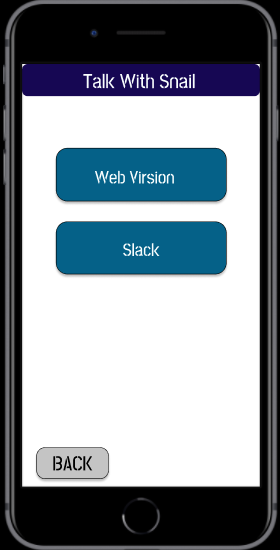
\includegraphics[width=0.4\linewidth]{chap4/image4/chat.png}
  \caption[Interactive Chatbot (Snail) activity Component ]{Interactive Chatbot (Snail) activity Component\index{Hasnain}}
  \label{fig:chat}
\end{figure}

Also known as a chatbot is a \acf{ACE}, chat robot, talk bot, chatterbot, or chatterbox. In our thesis, we used chatbot as trusted in the workplace. In figure \ref{fig:chat} shows the process diagram of chatbot activity. The chatbot will interactively talk with the user and suggest some activity for relaxation. 

I used two platforms to make this bot, one is web-based using React.\acs{js} and Dialogflow \acs{API}. Another one is Slack platform which most commonly used for corporate communication in the workplace. I integrate slack with Dialogflow \acs{API}.In figure: \ref{fig:Slackchat} shows the Slack Chatbot (Snail) Interface.

\begin{figure}[hbt!] 
  \centering
  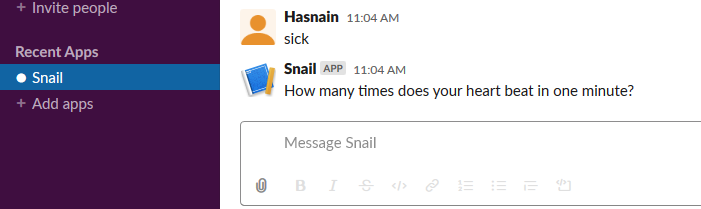
\includegraphics[width=1.0\linewidth]{chap4/image4/slack_chat.png}
  \caption[Slack Chatbot(Snail) Interface ]{Slack Chatbot(Snail) Interface\index{Hasnain}}
  \label{fig:Slackchat}
\end{figure}

Dialogflow is a Google-owned human-computer interaction technology company based on conversations in the natural language. The company is best known for creating the Assistant, a virtual mobile buddy for Android, iOS, and Windows Phone that performs tasks and answers user questions in a natural language.\citep{Zax2012TheSolved} Speaktoit has developed a natural language processing system that integrates the context of interaction such as dialogue history, location, and user preferences. This is the main reason we chose Dialogflow back-end for our system.

Use Dialogflow API A prototype chatbot called \textbf{Snail} has been developed to make access to a self-help library simpler for a more immersive user journey. The library of self-help consists of such categories as abuse of anxiety, depression, obesity, and alcohol/drug. That category contains numerous data files which contain information about each category. To find the information they are searching for, the user is expected to click in the various categories. The chatbot was designed to provide a more engaging way to lead the user to workplace stress relief and ask them what areas they would like information about.

In this activity, we build a system employs chatbots to conduct a conversation with individuals to derive a measure of stress using a Sense of Coherence conversation. The outputs of this conversation then drive an analysis dashboard which selects and administers an intervention intending to reduce measured stress. The conversation and Sense of Coherence conversation that we develop are capable of measuring stress and can be used by the analysis dashboard to successfully select appropriate support actions.

\section{Stress Analytic Dashboard}
In the firebase cloud database, I stored activity metadata about the sensors and chatbot interaction, which is not understandable, which annotations are wrong. Visualize the sensor and chatbot interaction data and the annotated information with it I used \acf{js} based visualization tool, which helps users. Therefore, the user can understand, when and what was the stress level during the working time. So the user can take appropriate measures when stress overflow and monitor users activity. The activity dashboard feature of our system for visualizing data is shown by the following figure.
\begin{figure}[hbt!] 
  \centering
  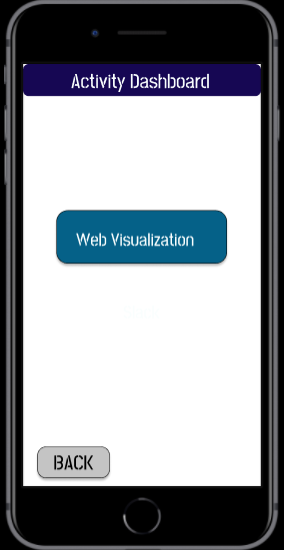
\includegraphics[width=0.4\linewidth]{chap4/image4/dashboard.png}
  \caption[Stress Analytics Dashboard Activity ]{Stress Analytic Dashboard Activity\index{Hasnain}}
  \label{fig:dashboard}
\end{figure}
Activity Analysis dashboards can be used for a variety of purposes, including strategy analysis and execution, performance reviews, performance improvement, data comprehension, and scope opportunity. But why is the format better than other visualizations of the data? Here are three main benefits of the Stress Management dashboards:
\subsubsection*{Access \& Understand Data:}
An Activity dashboard summarizes and visualizes data in a way that makes it easy to understand what’s important and what needs immediate attention. It shows personal performance at a glance. From there, users can make quick analyses and take action with confidence, backed by data. 
\subsubsection*{Predict Trends:}
Providing a high-level, graphic view of a facility’s numbers helps the empowerment spot trends. A dashboard shows if a \acs{KPI} is tracking above or below its benchmark over time in the workplace. User can make predictions and quickly adjust the strategy or goals when needed.
\subsubsection*{Prioritize:}
Another benefit of dashboards in Activity Analytic is they display individuals most essential data. User can drill down into any \acs{KPI} to get more information, but everything is rolled up into high-level goals. This helps establish priorities because you can see how the minute data affects the larger goals.

Activity Analytics Dashboard offers you a comprehensive view of the data. User needs to focus on areas that need immediate attention while filtering out distractions.

\begin{figure}[hbt!] 
  \centering
  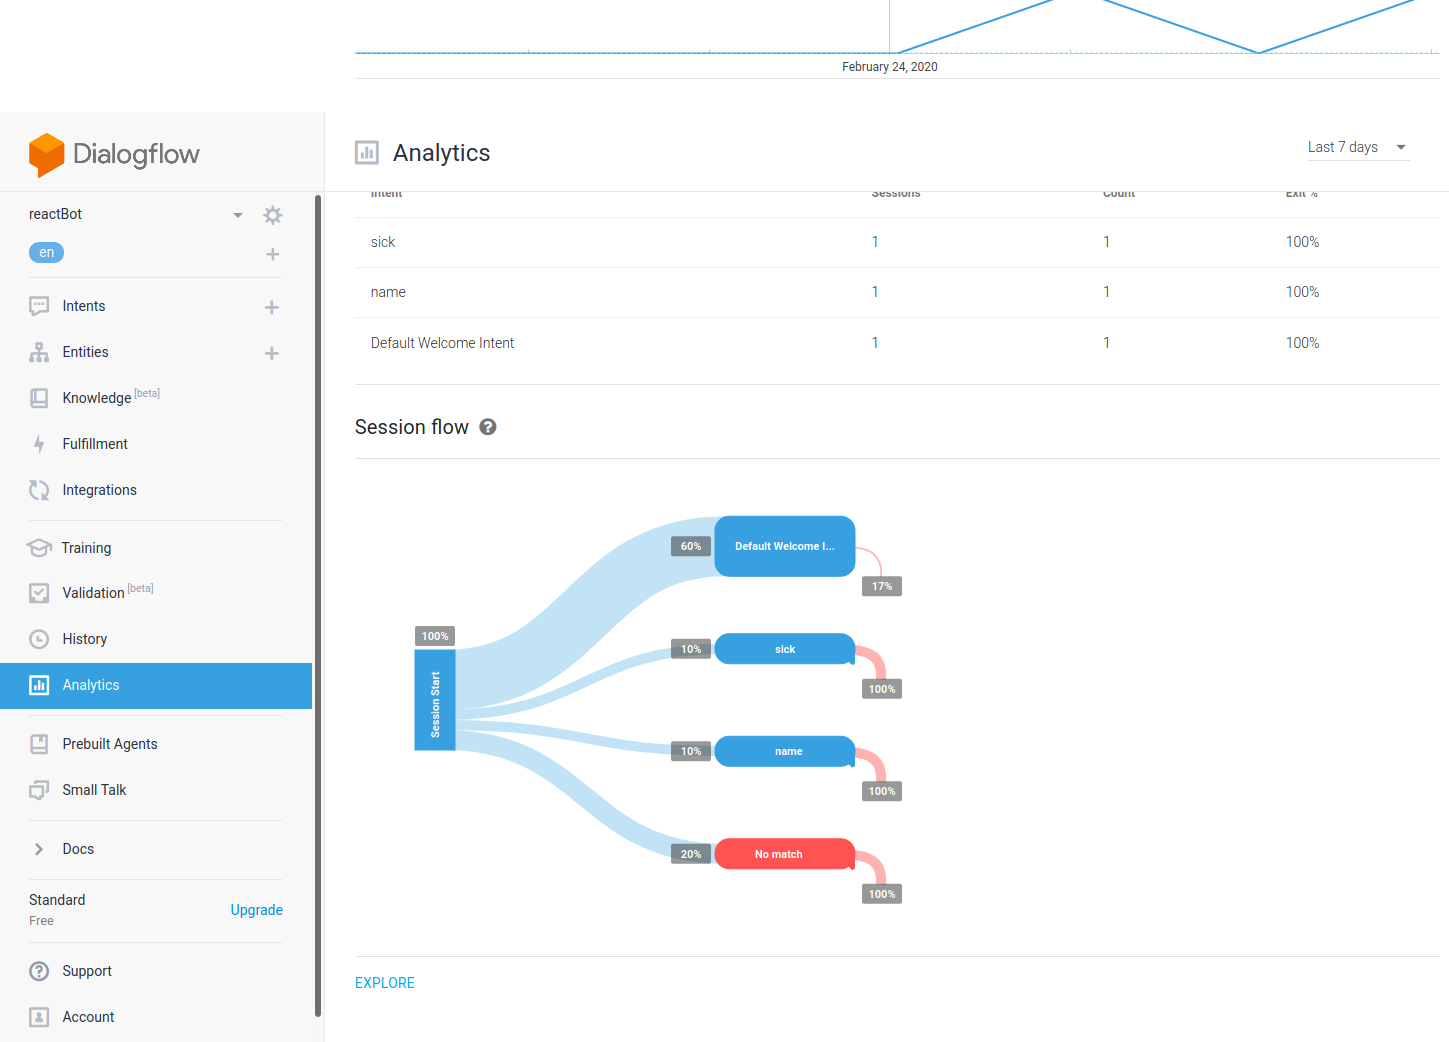
\includegraphics[width=1.0\linewidth]{chap4/image4/flow2.png}
  \caption[Dialogflow chatbot session activity visualization ]{Dialogflow chatbot session activity visualization\index{Hasnain}}
  \label{fig:flow2}
\end{figure}

In this activity, I develop an Activity Analytics Dashboard using react.js and Dialogflow API to analyze the activity of Stress Overflowed people in the workplace.  In figure \ref{fig:flow2} shows the one session chatbot activity visualization at Dialogflow.

To sum up; this chapter has discussed the development of the system for this study. I have addressed the process, activity and development tools. Afterwards, the next chapter of the thesis will discuss the experiment and result that I have gotten from the prototype experiment by the participant.


